\chapter{Day 2: Matrix Transformations}

\section{Schedule}
\begin{itemize}
\item 0900-0915: Debrief
\item 0915-0945: Synthesis
\item 0945-1030: 2D Rotations
\item 1030-1045: Coffee
\item 1045-1130: 3D Rotations
\item 1130-1200: Reflections and Shearing
\item 1200-1220: Review and Preview
\item 1220-1230: Survey
\end{itemize}

\section{Debrief}

\begin{itemize}

\item With your table-mates, identify a list of key concepts/take home messages/things you learned in the assignment. Try to group them in categories like "Concepts", "Technical Details", "Matlab", etc.

\item Try to resolve your confusions with your table-mates and by talking to an instructor.

\end{itemize}

\section{Synthesis}

\begin{prob}
These are fundamental ideas about matrices and it is important to complete these. They should be done by hand.
\be
\item What is the difference between a scalar, a vector, a matrix, and an array?
\item What are the rules for adding matrices?
\item When can two matrices be multiplied, and what is the size of the output?
\item What is the distributive property for matrix multiplication?
\item What is the associative property for matrix multiplication?
\item What is the commutative property for matrix multiplication?
\ee
\end{prob}
\begin{sol}
\be
\item Scalars, vectors, and matrices are examples of arrays. A 0-dimensional array can be thought of as a scalar. A 1-dimensional array is a vector. A 2-dimensional array is a matrix.
\item The matrices have to be the same size and addition is element-wise.
\item The matrices have to compatible (inner dimensions agree), and the output is dictated by the outer dimensions, i.e. $(n \times m) (r \times s) = (n \times s)$.
\item Distributive property: $\mathbf{A} (\mathbf{B} + \mathbf{C}) = \mathbf{A} \mathbf{B} + \mathbf{A} \mathbf{C}$
\item Associative property: $\mathbf{A} (\mathbf{B} \mathbf{C} ) = (\mathbf{A} \mathbf{B}) \mathbf{C}$
\item Commutative property:
Two matrices commute if $\mathbf{A} \mathbf{B} = \mathbf{B} \mathbf{A}$ but this is not always true.
\ee
\end{sol}

\begin{prob}
These are synthesis problems. It would be helpful to complete these. They should be done by hand.
\be
\item Consider the matrix $\A = \twobytwo{1}{2}{3}{4}$. Show that $\A^2$ commutes with $\A$. 
\item Use the distribution law to expand $(\A + \mathbf{B})^2$ assuming that $\A$ and $\mathbf{B}$ are matrices of appropriate size. How does this compare to the situation for real numbers?
\item Show that $\mathbf{D} = \twobytwo{4}{-2}{3}{-3}$ satisfies the matrix equation $\mathbf{D}^2 - \mathbf{D} - 6 \mathbf{I} = \mathbf{0}$.
\ee
\end{prob}
\begin{sol}
\be
\item You need to show that $\A^2 \A = \A \A^2$ for this particular matrix. You can do it by multiplying.
\item Using the distributive property  you can see that $(\mathbf{A} + \mathbf{B})^2 = (\mathbf{A} + \mathbf{B}) ( \mathbf{A} + \mathbf{B}) = \mathbf{A}^2 + \mathbf{AB} + \mathbf{BA} + \mathbf{B}^2$
\item If you plug $\mathbf{D}$ and $\mathbf{D}^2$ into the equation you should find that the result is a zero matrix.
\ee
\end{sol}

\begin{prob}
These are challenge problems. Pick one of them to wrestle with. It is not important to complete these. They should be done by hand.
\be
\item The matrix exponential is defined by the power series
\[ \exp{\A} = \sum_{k=0}^{\infty} \frac{\A^k}{k!} \]
Assume $\A = \twobytwo{2}{0}{0}{3}$. Find a formula for $\exp{\A}$. 
\item The real number $0$ has just one square root: $0$. Show, however, that the $2 \times 2$ zero matrix has infinitely many square roots by finding all $2 \times 2$ matrices $\mathbf{A}$ such that $\mathbf{A}^2 = \mathbf{0}$.  
\item Use induction to prove that $\A^n$ commutes with $\A$ for any square matrix $\A$ and positive integer $n$.
\ee
\end{prob}
\begin{sol}
\be
\item The matrix exponential is defined by the power series $\exp{\A} = \mathbf{I} + \A + \frac{\A^2}{2!} + \ldots$. Notice that this $\A$ is diagonal and $\A^2 = \twobytwo{2^2}{0}{0}{3^2}$ and the exponential becomes $\exp{\A} = \twobytwo{1 + 2 + 2^2/2! + \ldots}{0}{0}{1 + 3 + 3^2/2! + \ldots}$. If you have seen power series before then you will recognise that $\exp{\A} = \twobytwo{\exp{2}}{0}{0}{\exp{3}}$.
\item You can define a general two by two matrix $\A = \twobytwo{a}{b}{c}{d}$, find $\A^2$, set each of the entries equal to zero and find constraints on the entries $a,b,c,d$.
\item You need to show that $\A^n \A = \A \A^n$ for any square matrix $\A$ and any positive integer $n$ by induction. First you show it is true for $n=1$ and $n=2$. Then assume it is true for some $n=k$, and prove that it must be true for $n=k+1$. You use the fact that $\A$ commutes with itself and the associative property, i.e $ \A^2 \A = (\A \A) \A = \A (\A \A) = \A \A^2$.
\ee
\end{sol}

% \item Suppose that you had a matrix  $\mathbf{A}$ which represents grayscale values corresponding to an image. Together with your table, convince yourselves that the if the matrix $\mathbf{E}$ defined below had the appropriate dimensions, the product $\mathbf{EA}$ would be an image for which the edges would be enhanced, i.e. $\mathbf{E}$ can function as an edge-detection matrix.

%     \begin{align*}
% \mathbf{E} =
% \begin{pmatrix}
%     1 & -1 & 0 & \cdots & \cdots &  0\\
%     0 & 1 &  -1 & 0 & \cdots & 0  \\
%     \vdots & \cdots & \ddots &\ddots & \cdots & \vdots & \\
%     -1 & \cdots & \cdots& \cdots & \cdots & 1
%  \end{pmatrix}
% \end{align*}

% Open up MATLAB, and load giraffe.mat. This file contains a picture of a giraffe stored as a grayscale image. You can display it by running  {\tt >> %imagesc(giraffe); colormap('gray');}. Verify that the above is true by applying $\mathbf{E}$ to the giraffe image.

\section{2D Rotation Matrices}
We're going to think about how to use rotation matrices to rotate a geometrical object. In doing so we will solidify fundamental concepts around matrix multiplication and start to explore the notion of ``inverse''. For clarity we will first work in 2D. Recall that the rotation matrix $\R(\theta)$:
\[ \R(\theta) = \twobytwo{\cos \theta}{-\sin \theta}{\sin \theta}{\cos \theta} \]
will rotate an object counterclockwise \textbf{about the origin} through an angle of $\theta$.

\begin{prob}
This is a hands-on, conceptual problem involving the multiplication of 2D rotation matrices. 
\be
\item Place an object on your table, and imagine that the origin of an xy-coordinate system is at the center of your object with $+z$ pointing upwards. 
\item Rotate it counterclockwise by 30 degrees, and then again by another 60 degrees. What is it's orientation now? How would you get there in one rotation instead? What does this suggest about the multiplication of rotation matrices?
\item What happens if you first rotate it by 60 degrees, and then by 30 degrees? What does this suggest about the commutative property of 2D rotation matrices?
\ee
\end{prob}

\begin{sol}
\be
\item Okay, I placed my book on the table.
\item You could get there by rotating once by 90 degrees. This suggests that the product of two rotation matrices of angles $\theta_1$ and $\theta_2$ is a rotation matrix of $\theta_1+\theta_2$, i.e. $\R(\theta_1) \R(\theta_2) = \R(\theta_1+\theta_2)$.
\item You end up in the same orientation so it doesn't matter the order. This suggests that the order of multiplication doesn't matter so that two rotation matrices must commute.
\ee
\end{sol}

\begin{prob}
This is an algebra problem involving the multiplication of 2D rotation matrices.
\be
\item Use some algebra to show that 2D rotation matrices commute, i.e. $\R(\theta_1) \R(\theta_2) = \R(\theta_2) \R(\theta_1)$.
\item Use some algebra to show that $\R(\theta_1) \R(\theta_2) = \R(\theta_1+\theta_2)$. You will need to look up some trig identities.
\ee
\end{prob}

\begin{sol}
\be
\item You could multiply out two rotation matrices with angle $\theta_1$ and $\theta_2$ in the two different orders and you will observe that the output is the same because real numbers commute, i.e. $\cos \theta_1 \cos \theta_2 = \cos \theta_2 \cos \theta_1$.
\item If you multiply two matrices together you will get the following expression in the first row and first column, $\cos \theta_1 \cos \theta_2 - \sin \theta_1 \sin \theta_2$. You will find a trig identity which reduces this to $ \cos (\theta_1 + \theta_2)$. Similar reductions take place for the other elements.
\ee
\end{sol}


\begin{prob}\label{ex:rotation}
Now, consider a rectangle of width 2 and height 4, centered at the origin. For clarity, this means that the corners of the rectangle have coordinates $(1,2)$, $(-1,2)$, $(-1,-2)$, and $(1,-2)$. 
\begin{enumerate}
\item Plot these four points by hand and connect them with lines to complete the rectangle.
\item Now, using the appropriate rotation matrix, transform each of the corner points by a rotation through 30 degrees counterclockwise (recall that the sin and cos of 30 degrees can be expressed exactly).  Compute and plot the resulting points by hand and connect them with lines.  Does the resulting figure look like you'd expect?
\end{enumerate}
\end{prob}
\begin{sol}
\begin{enumerate}
    \item The rectangle is
    \begin{center}
    \begin{tikzpicture}[scale=.3]
    \draw [->,gray!50!black] (0,0)--(0,3) node[above]{$y$};
    \draw [->,gray!50!black] (0,0)--(3,0) node[right]{$x$};
    \draw [red] (1,2)--(1,-2)--(-1,-2)--(-1,2)--(1,2);
    \end{tikzpicture}
    \end{center}
    
    \item The rotation matrix is
    $$\mathbf{R} = \begin{bmatrix}
    \cos 30 & -\sin 30 \\ \sin 30 & \cos 30
    \end{bmatrix} = \begin{bmatrix}
    \frac{\sqrt{3}}{2} & -\frac12 \\ \frac12 & \frac{\sqrt{3}}{2}
    \end{bmatrix}.$$
    Applying this to each point, we get
    $$\mathbf{R}\begin{bmatrix}
    1 \\ 2
    \end{bmatrix} = \begin{bmatrix}
    \frac{\sqrt{3}-2}{2} \\ \frac{1 + 2\sqrt{3}}{2}
    \end{bmatrix}, \
    \mathbf{R}\begin{bmatrix}
    1 \\ -2
    \end{bmatrix} = \begin{bmatrix}
    \frac{\sqrt{3}+2}{2} \\ \frac{1 - 2\sqrt{3}}{2}
    \end{bmatrix},$$
    $$\mathbf{R}\begin{bmatrix}
    -1 \\ 2
    \end{bmatrix} = \begin{bmatrix}
    \frac{-\sqrt{3}-2}{2} \\ \frac{-1 + \sqrt{3}}{2}
    \end{bmatrix}, \
    \mathbf{R}\begin{bmatrix}
    -1 \\ -2
    \end{bmatrix} = \begin{bmatrix}
    \frac{-\sqrt{3}+2}{2} \\ \frac{-1 - \sqrt{3}}{2}
    \end{bmatrix}.$$
    And the rotated figure looks like,
    \begin{center}
    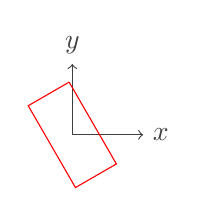
\begin{tikzpicture}[scale=.3]
    \draw [->,gray!50!black] (0,0)--(0,3) node[above]{$y$};
    \draw [->,gray!50!black] (0,0)--(3,0) node[right]{$x$};
    \draw [red] (-0.134,2.2321)--(1.866,-1.2321)--(0.1340,-2.2321)--(-1.866,1.2321)--(-0.134,2.2321);
    \end{tikzpicture}
    \end{center}
\end{enumerate}
\end{sol}

\begin{prob}
Now, let's do it in MATLAB. 
\begin{enumerate}
\item Create and plot the original 4 points:$(1,2)$, $(-1,2)$, $(-1,-2)$, and $(1,-2)$. Then create the matrix that rotates them by 30 degrees counterclockwise, transform each of the four original points using the rotation matrix, and plot the resulting points.  Does this look right? \textit{Reminder: \texttt{plot(1,2,`x')} puts a mark at the point (1,2)}. \textit{Matlab: the functions cos and sin expect radians, while cosd and sind expect degrees.}
\item  Operating on individual points with the rotation matrix is cool, but we can be much more efficient by operating on all 4 points at the same time. Write down the matrix whose columns represent the four corners of the rectangle. Then write down the matrix multiplication problem we can solve to transform the rectangle from above all at once.  Create these matrices in MATLAB to perform the rotation in a single operation.  Plot the resulting matrix to confirm your transformation!	\textit{Some MATLAB tips: \texttt{plot(X,Y)} creates a line plot of the values in the vector \texttt{Y} versus those in the vector \texttt{X}.  So if you wanted to plot a line from the origin (0,0) to the point (1,2), you would do this: \texttt plot([0 1],[0 2])}.  The command \texttt{axis([-xlim xlim -ylim ylim])} sets the axes of the current plot to run from \texttt{-xlim} to \texttt{xlim} and  from \texttt{-ylim} to \texttt{ylim}
\item What is the area of the rectangle before and after the rotation?
\item What matrix should you use to undo this rotation? Define it in MATLAB and check.
\item Show on the board that the product of this matrix with the original rotation matrix is the identity matrix. For clarity, let's give this matrix the symbol $\R^{-1}$. It is the matrix that inverts the original operation and is known as the \textit{inverse} of the matrix $\R$.
%\item EXTRA FUN( if you have time): A 2D boat occupies the region defined by $x^2/2 < y < 2$. What is the region definition If we want to rotate the boat counterclockwise by angle $\theta$ about the origin? 
%\item BONUS FUN (if you have extra time): Modify your MATLAB script to create an animation of a rotating rectangle. (The commands $\it{drawnow}$ and $\it{pause}$ are your friends. You might need to do this outside of the notebook Live Editor or pop out your figure.)
\end{enumerate}
\end{prob}
\begin{sol}
\begin{enumerate}
    \item There are lots of ways to do this point by point. Here is an example of how to transform the bottom right point:
    \begin{verbatim}
    >> BR = [1;-2]
    >> plot(BR(1,:),BR(2,:),'b*')
    >> rotmatrix = [cosd(30) -sind(30); sind(30) cosd(30)]
    >> nBR = rotmatrix*BR
    >> plot(nBR(1,:),nBR(2,:),'r*')
    \end{verbatim}
    
    \item There are lots of ways to do this. Here is an example where we include the first point twice so that the points can easily be connected with lines:
    \begin{verbatim}
    >> pts = [1 -1 -1 1 1;2 2 -2 -2 2]
    >> npts = rotmatrix*pts
    >> plot(pts(1,:),pts(2,:),'b'), hold on
    >> plot(pts(1,:),pts(2,:),'r')
    >> axis([-3 3 -3 3])
    >> axis equal
    \end{verbatim}
    
    \item The area of the rectangle is the same before and after rotation: 8 square units.
    
    \item To undo this rotation you could simply rotate it by 30 degrees clockwise, using the matrix
    $$\mathbf{R}^{-1} = \begin{bmatrix}
    \cos 30 & \sin 30 \\ -\sin 30 & \cos 30
    \end{bmatrix}.$$
    
    \item The product of $\mathbf{R}^{-1}$ and $\mathbf{R}$ is
    $$\mathbf{R}^{-1} \mathbf{R} = \twobytwo{\cos \theta}{\sin \theta}{-\sin \theta}{\cos \theta} \twobytwo{\cos \theta}{-\sin \theta}{\sin \theta}{\cos \theta} = \twobytwo{\cos^2 \theta + \sin^2 \theta}{0}{0}{\cos^2 \theta + \sin^2 \theta} = \twobytwo{1}{0}{0}{1}$$
    where we have used the trig identity $\cos^2 \theta + \sin^2 \theta = 1$.

\end{enumerate}
\end{sol}

\section{3D Rotations}

We can extend the idea of 2D rotations to 3D rotations. The simplest approach is to think of 3D rotations as a composition of rotations about different axes. First let's define the rotation matrices for counterclockwise rotations of angle $\theta$ about the $x, y$ and $z$ axes respectively.
\begin{align}
\R_{x} &= \begin{bmatrix}
1 & 0 & 0 \\
0 & \cos \theta &  -\sin \theta \\[3pt]
0 & \sin \theta  &  \cos \theta \\[3pt]
\end{bmatrix} \\[6pt]
\R_{y} &= \begin{bmatrix}
\cos \theta & 0 & \sin \theta \\[3pt]
0 & 1 & 0 \\[3pt]
-\sin \theta & 0 & \cos \theta \\
\end{bmatrix} \\[6pt]
\R_{z} &= \begin{bmatrix}
\cos \theta &  -\sin \theta & 0 \\[3pt]
\sin \theta &   \cos \theta & 0\\[3pt]
0 & 0 & 1\\
\end{bmatrix}
\end{align}
For example, to first rotate a vector $\mathbf{v}$ counterclockwise by $\theta$ about the $x$ axis followed by counterclockwise by $\phi$ about the $z$ axis, you need to do the following
\begin{align}
\begin{bmatrix}
\cos \phi &  -\sin \phi & 0 \\[3pt]
\sin \phi &   \cos \phi & 0 \\[3pt]
0 & 0 & 1\\
\end{bmatrix}
\begin{bmatrix}
1 & 0 & 0 \\
0 & \cos \theta &  -\sin \theta \\[3pt]
0 & \sin \theta  &  \cos \theta \\[3pt]
\end{bmatrix}
\mathbf{v}
\end{align}


We will next look at some sequence of physical rotations and relate them to these rotation matrices.

\begin{prob}
Hold a closed book in front of you, with the top of the book towards the ceiling ($+z = (0,0,1)$ direction) and the cover of the book pointed towards you ($+x = (1,0,0)$ direction), which leaves the opening side of the book pointing towards your right ($+y = (0,1,0)$) and the spine toward the left.
    \begin{enumerate}
    \item  Rotate the book by 90 degrees counter-clockwise about the $x$-axis, then from this position, rotate the book by 90 degrees counter-clockwise about the $z$-axis.  Which direction is the cover of the book facing now?
    \item  Return to the starting position.  Now rotate the book by 90 degrees counter-clockwise about the $z$ axis, and then from this position, rotate the book by 90 degrees counter-clockwise about the $x$ axis.  Which direction is the cover of the book facing now?  Is it the same as in part a?
    \item  An operation "commutes" if changing the order of operation doesn't change the result. Do 3D rotations commute? 
    \item  The cover of the book is originally pointed towards $(1,0,0)$.  Multiply this vector with the appropriate sequence of rotation matrices from above to reproduce your motions from part 1.  Do you end up with the correct final cover direction?
    \item  Multiply the $(1,0,0)$ vector with the appropriate sequence of rotation matrices to reproduce the motions from part 2.  Do you end up with the correct final cover direction?
    \item Multiply the result of the previous part by the appropriate sequence of rotation matrices to return to the original $(1,0,0)$ vector.
    \item  From either of your answers to part 4 or part 5, try, instead of operating on the $(1,0,0)$ vector sequentially with one rotation matrix and then the other, take the product of the two rotation matrices first, and then multiply $(1,0,0)$ with the resultant matrix.  Does this reproduce your answer?
    \item Based on your answers to the previous parts, show that $\left(\R_z \R_x\right)^{-1} = \R_x^{-1} \R_z^{-1}$. This is a general property of matrix inverses -- it works for all square, invertible matrices, not just rotation matrices!
    \end{enumerate}
\end{prob}
\begin{sol}
\begin{enumerate}
    \item The cover is now facing toward the $+y$ axis (the positive part of the $y$ axis).
    \item The cover is now facing the $+z$ axis. This is different than in part a.
    \item Since the answers for the first two parts are different, 3D rotations do not commute.
    \item Let $\mathbf{v}$ be the vector that represents the initial direction of the cover of the book,
    $$\mathbf{v} = \begin{bmatrix}
    1 \\ 0 \\ 0
    \end{bmatrix}.$$
    Rotation by 90 degrees counterclockwise around the $x$ axis is given by
    $$\mathbf{R}_x = \begin{bmatrix}
    1 & 0 & 0 \\
    0 & 0 &  -1 \\[3pt]
    0 & 1  &  0 \\[3pt]
    \end{bmatrix}.$$
    so that the new vector becomes 
    $$\mathbf{R}_x \mathbf{v} = \threebyone{1}{0}{0}$$
    Rotation by 90 degrees counterclockwise around the $z$ axis is given by
    $$\mathbf{R}_z = \begin{bmatrix}
    0 &  -1 & 0 \\[3pt]
    1 &   0 & 0\\[3pt]
    0 & 0 & 1\\
    \end{bmatrix}$$
    so that the new vector becomes
    $$\mathbf{R}_z \mathbf{R}_x \mathbf{v} = \threebyone{0}{1}{0}$$
    which is the correct final direction.
    
    \item Using the matrices from above,
    $$\mathbf{R}_x\mathbf{R}_z\mathbf{v} = \begin{bmatrix}
    0 \\ 0 \\ 1
    \end{bmatrix}.$$
    
    \item To rotate 90 degrees clockwise around the $x$ axis we use the matrix
    $$\mathbf{R}_x^{-1} = \begin{bmatrix}
    1 & 0 & 0 \\ 0 & 0 & 1 \\ 0 & -1 & 0
    \end{bmatrix}$$
    and to rotate 90 degrees clockwise around the $z$ axis we use the matrix $$\mathbf{R}_z^{-1} = \begin{bmatrix}
    0 & 1 & 0 \\ -1 & 0 & 0 \\ 0 & 0 & 1
    \end{bmatrix}.$$
    Then we can return the vector $(0,0,1)$ to its original position $(1,0,0)$ by
    $$\mathbf{R}_z^{-1}\mathbf{R}_x^{-1} \begin{bmatrix}
    0 \\ 0 \\ 1
    \end{bmatrix} = \begin{bmatrix}
    1 \\ 0 \\ 0
    \end{bmatrix}.$$
    
    \item We can multiply the rotation matrices together and perform a single matrix multiplication. For part d, the relevant matrix product is
    $$\mathbf{R}_z \mathbf{R}_x = \threebythree{0}{0}{1}{1}{0}{0}{0}{1}{0}$$
    and we see that
    $$\mathbf{R}_z \mathbf{R}_x \threebyone{1}{0}{0} = \threebyone{0}{0}{1}$$
    as expected. 
    
    \item We can see from the previous parts that
    $$(\mathbf{R}_z\mathbf{R}_x)^{-1} = \mathbf{R}_x^{-1}\mathbf{R}_z^{-1}.$$
    In other words, when you take the inverse, the order of operations must swap!
\end{enumerate}
\end{sol}

% JBG: I've removed this problem because I don't think we need it and we don't really have time.
% \begin{prob}
% Define a set of points in MATLAB that correspond to the corners of a cube in 3D - you can use \texttt{plot3} to visualize these. Now use the rotation matrix to rotate the cube counter-clockwise about an axis, and visualize this in MATLAB. 
% \end{prob}
% \begin{sol}
% to do
% \end{sol}

\section{Reflection and Shearing}

In this activity we will meet reflection and shearing matrices, which will allow us to explore transformation matrices in general.

\subsection{Reflection}

\begin{prob}
What do the following \textit{reflection} matrices do? Think about it first, draw some sketches and then test your hypothesis in MATLAB using the rectangle with vertices $(0,0), (2,0), (2,1),$ and $(0,1)$. How much does the area of your basic rectangle change, if at all? What is the inverse of each?
\begin{enumerate}
\item \[ \twobytwo{-1}{0}{0}{1} \]
\item \[ \twobytwo{1}{0}{0}{-1} \]
\item \[ \twobytwo{\cos 2\theta}{\sin 2\theta}{\sin 2\theta}{-\cos 2\theta} \]
\end{enumerate}
\end{prob}
\begin{sol}
\begin{enumerate}
    \item This matrix reflects everything over the $y$-axis. In the figure below, the original blue rectangle becomes the orange rectangle. The area of the rectangle stays the same.
    \begin{center}
        \includegraphics[width=.75\textwidth]{FacesDay2/figs/yreflect.jpg}
        \captionof{figure}{Reflection over $y$-axis.}
        \label{fig:yreflect}
    \end{center}
        \item This matrix reflects everything over the $x$-axis. In the figure below, the original blue rectangle becomes the orange rectangle. The area of the rectangle stays the same.
    \begin{center}
        \includegraphics[width=.75\textwidth]{FacesDay2/figs/xreflect.jpg}
        \captionof{figure}{Reflection over $x$-axis.}
        \label{fig:xreflect}
    \end{center}
    \item For example, let $\theta=30$ degrees. Then the rectangle is reflected along the line that is 30 degrees counterclockwise from the $x$-axis. In the figure below, the original blue rectangle becomes the orange rectangle.
    \begin{center}
        \includegraphics[width=.75\textwidth]{FacesDay2/figs/reflect.jpg}
        \captionof{figure}{Reflection over 30 degree line.}
        \label{fig:reflect}
    \end{center}
    Notice that, if we plug in $\theta=90$, we get the matrix from part 1, which reflects over the $x$-axis (i.e., 90 degree line) and, if we plug in $\theta=0$, we get the matrix from part 2, which reflects over the $y$-axis (i.e., the 0 degree line).
\end{enumerate}
\end{sol}

\subsection{Shearing}

\begin{prob}
What do the following \textit{shearing} matrices do? Think about it first, draw some sketches and then test your hypothesis in MATLAB with the rectangle with vertices $(0,0), (2,0), (2,1),$ and $(0,1)$. How much does the area of your basic rectangle change, if at all? What is the inverse of each?
\begin{enumerate}
\item \[ \twobytwo{1}{1}{0}{1} \]

\item \[ \twobytwo{1}{0}{1}{1} \]

\item \[ \twobytwo{1}{2k}{0}{1} \]

\item \[ \twobytwo{1}{0}{2k}{1} \]
\end{enumerate}
\end{prob}
\begin{sol}
\begin{enumerate}
    \item This shearing matrix pulls the points along horizontal lines and the strength of the pull is proportional to the $y$ coordinate. In the figure below, the blue rectangle is sheared to become the orange rectangle:
        \begin{center}
        \includegraphics[width=.75\textwidth]{FacesDay2/figs/xshear.jpg}
        \captionof{figure}{Shearing in $x$ direction.}
        \label{fig:xshear}
    \end{center}
    The area of the rectangle does not change. The inverse is
    $$\begin{bmatrix}
    1 & -1 \\ 0 & 1
    \end{bmatrix}.$$
    
        \item This shearing matrix pulls the points along vertical lines and the strength of the pull is proportional to the $x$ coordinate. In the figure below, the blue rectangle is sheared to become the orange rectangle: 
        \begin{center}
        \includegraphics[width=.75\textwidth]{FacesDay2/figs/yshear.jpg}
        \captionof{figure}{Shearing in $y$ direction.}
        \label{fig:yshear}
    \end{center}
        The area of the rectangle does not change. The inverse is
    $$\begin{bmatrix}
    1 & 0 \\ -1 & 1
    \end{bmatrix}.$$
    
        \item This shearing matrix pulls the points along horizontal lines and the strength of the pull is proportional to the $y$ coordinate and the constant $k$ (the bigger the $k$, the stronger the pull). In the figure below, with $k=2$, the blue rectangle is sheared to become the orange rectangle: 
        \begin{center}
        \includegraphics[width=.75\textwidth]{FacesDay2/figs/bigxshear.jpg}
        \captionof{figure}{Shearing in $x$ direction with $k=2$.}
        \label{fig:bigxshear}
    \end{center}
    The area of the rectangle does not change. The inverse is
    $$\begin{bmatrix}
    1 & -4 \\ 0 & 1
    \end{bmatrix}.$$
    
        \item This shearing matrix pulls the points along vertical lines and the strength of the pull is proportional to the $x$ coordinate and the constant $k$ (the bigger the $k$, the stronger the pull). In the figure below, with $k=2$, the blue rectangle is sheared to become the orange rectangle: 
        \begin{center}
        \includegraphics[width=.75\textwidth]{FacesDay2/figs/bigyshear.jpg}
        \captionof{figure}{Shearing in $y$ direction with $k=2$.}
        \label{fig:bigyshear}
    \end{center}
        The area of the rectangle does not change. The inverse is
    $$\begin{bmatrix}
    1 & 0\\ -4 & 1
    \end{bmatrix}.$$
\end{enumerate}
\end{sol}

\section*{Review and Preview}
\begin{ournotes}
John's Review:
\bi
\item Matrices are holders of data, e.g. coordinates of points
\item Matrices are transformation operators, e.g. rotation, reflection, shearing.
\item Matrices have algebraic properties:
\bi
\item $\A + \B = \B + \A$
\item $(\A \B)\C = \A (\B \C)$
\item $\A \B \ne \B \A$ (don't always commute)
\ei
\item 2D Rotation Matrix (does commute)
\[\R(\theta) = \twobytwo{\cos \theta}{-\sin \theta}{\sin \theta}{\cos \theta}\]
\item 3D Rotation Matrices (do not commute about different axes)
\item Order of operations:
$\A \B \v$ implies that $\B$ acts on $\v$, and then $\A$ acts on the result.
\item Inverse Matrix: undoes a transformation
\bi
\item $\A^{-1} \A = \I$
\item $(\A \B)^{-1} = \B^{-1} \A^{-1}$
\ei
\ei
\end{ournotes}

\pagebreak
\shipoutAnswer


% \begin{prob}
% If you have extra time, here's some bonus fun: Consider the shearing matrix $\twobytwo{1}{2k}{0}{1}$. Try to decompose this into a rotation, a scaling, and another rotation. (This is not easy and may require lots of algebra)
% \end{prob}